% !TeX program = lualatex
% !TeX encoding = utf8

%\documentclass{beamer}
\documentclass[aspectratio=169, smaller]{beamer}

\usepackage{amsmath}
\usepackage[T1]{fontenc}

% This is the "normal" package based install
\usepackage{lhcb_presentation/ACATpackage}

\usepackage{units}
\usepackage{booktabs}
\usepackage{ulem}
\usepackage{comment}
\usepackage{listings}
\usepackage{pgfplots}
\usetikzlibrary{decorations.pathreplacing}
\pgfplotsset{compat=1.12}

\definecolor{ACATtan}{RGB}{201,159,109}
\definecolor{ACATdtan}{RGB}{179,72,18}
\definecolor{ACATlblue}{RGB}{24,146,200}
\definecolor{ACATdgreen}{RGB}{0,68,0}
\definecolor{ACATdbrown}{RGB}{65,14,23}
\definecolor{ACATbackground}{RGB}{255, 204, 102}

\tikzstyle{ACATdark}=[fill=ACATtan, draw=ACATdbrown, ultra thick]
\tikzstyle{ACATselected}=[fill=ACATdtan, draw=ACATdbrown, ultra thick]
\tikzstyle{ACATdarktext}=[text=ACATdbrown]
\tikzstyle{ACATselectedtext}=[text=white]

% This should be appendtographicspath if using package method
\appendtographicspath{{./images/}}

\lstset{
    columns=fullflexible,
    basicstyle=\ttfamily\small,
    stringstyle=\color{green!50!black},
    keywordstyle=\color{orange},
    commentstyle=\color{white!50!black},
    emph={GooFit,Observable,DataSet,UnbinnedDataSet,BinnedDataSet,
          Variable,FitManager,
          goofit,GaussianPdf,DalitzPlotter},
    emphstyle=\color{blue!50!black}
}

\errorcontextlines 10000

\title{A Python upgrade to the GooFit package for parallel fitting}

\author[Henry Schreiner]{%
        Henry Schreiner\textcolor{red}{\inst{1 }} \and
        Himadri Pandey\textcolor{red}{\inst{1 }} \and
        Michael Sokoloff\textcolor{red}{\inst{1 }} \and \\
        Hittle Bradley\textcolor{red}{\inst{2 }} \and
        Karen Tomko\textcolor{red}{\inst{2 }} \and
        Christoph Hasse\textcolor{red}{\inst{3 }}
}
\institute{\inst{1} University of Cincinnati \and
           \inst{2} Ohio Supercomputer Center \and
           \inst{3} CERN / Technische Universit{\"a}t Dortmund (DE)}
\date{\today}

% Auto-fullscreen
% \lhcbhypersetup

\begin{document}

\begin{frame}
\titlepage
\end{frame}

\section{GooFit Introduction}
\subsection{GooFit Introduction}
\begin{frame}{What is GooFit?}
    \begin{center}
        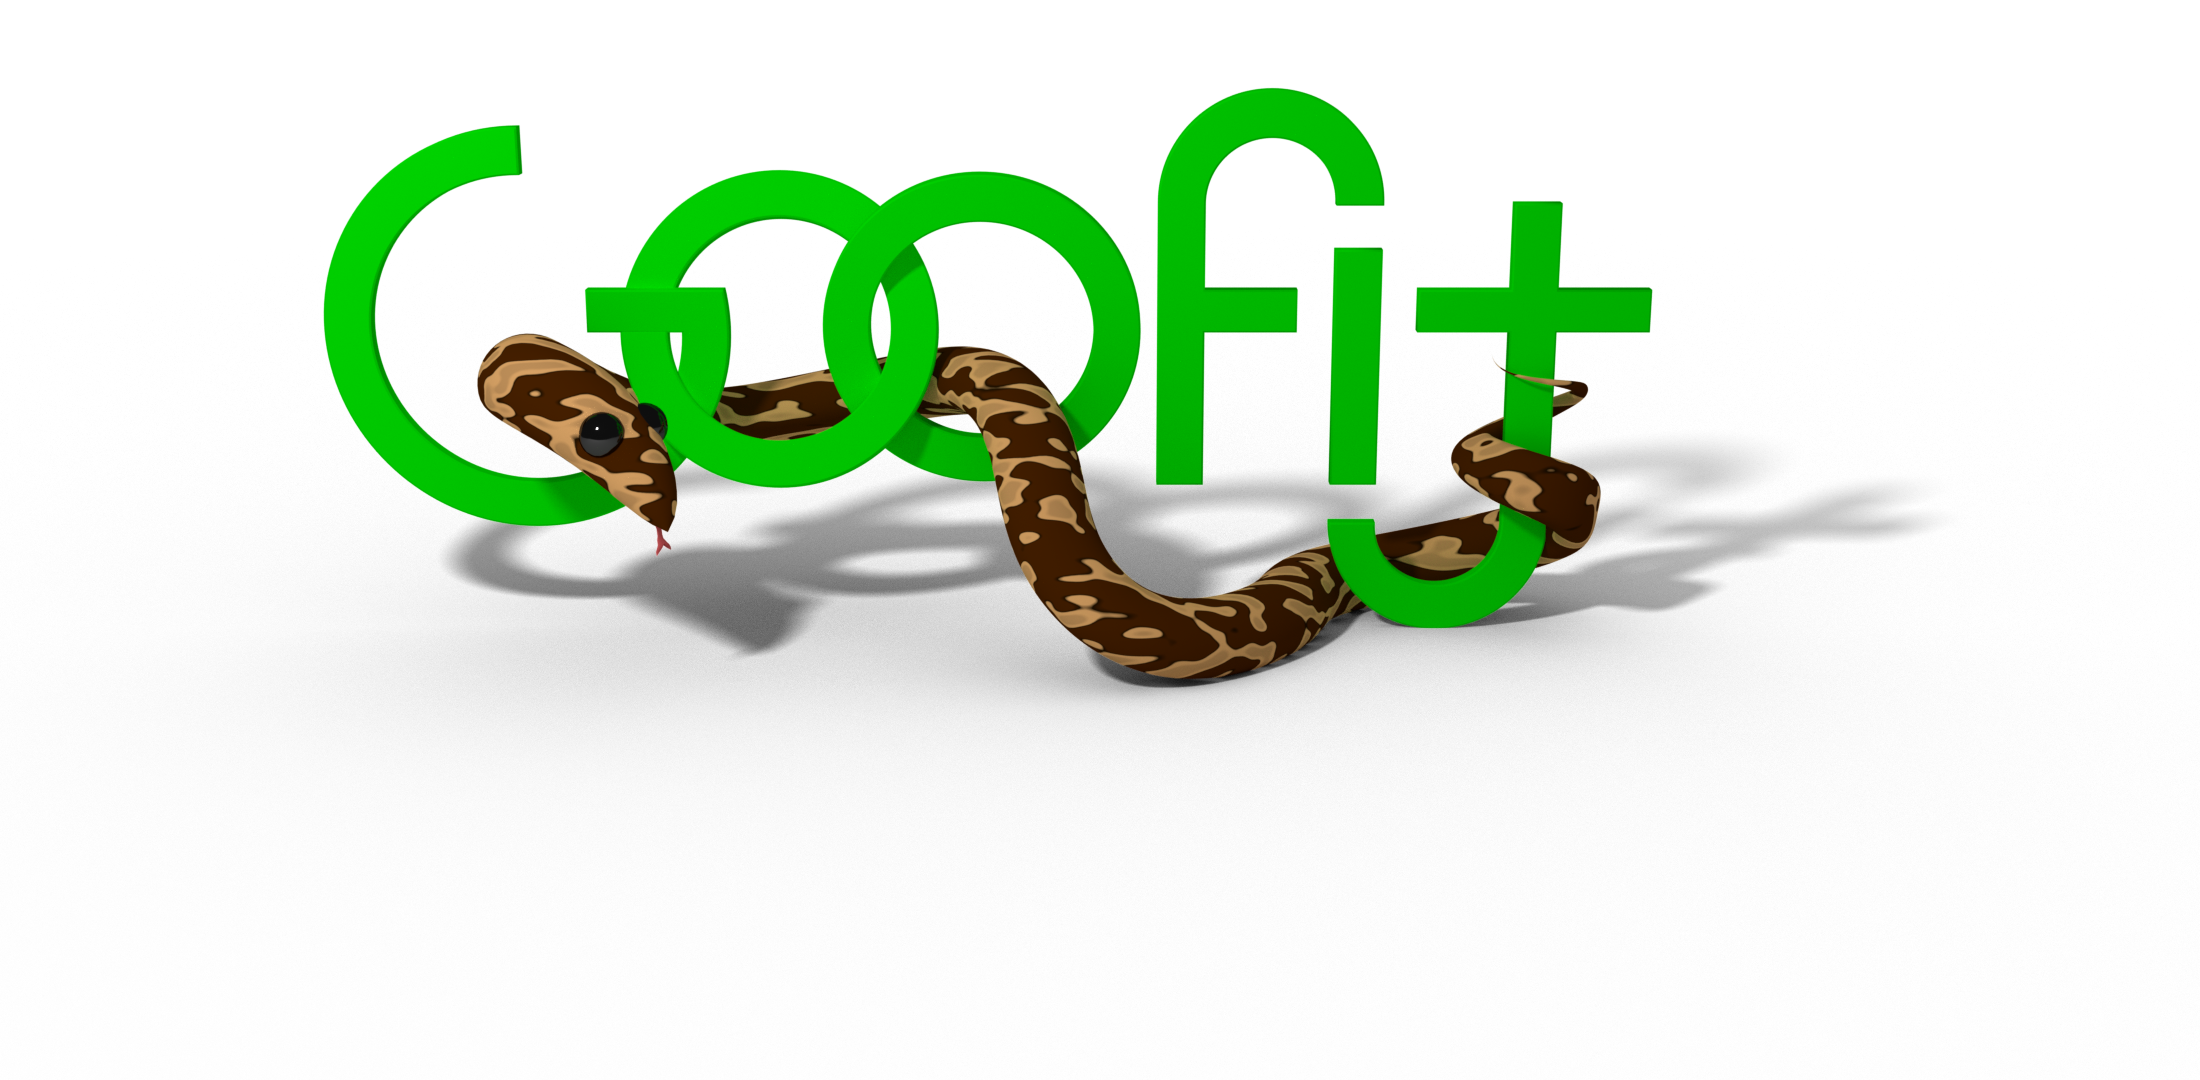
\includegraphics[width=0.7\textwidth, trim={100 450 300 200}]{GooFitSnake}
    \end{center}

    GPU and OpenMP embarrassingly parallel function evaluation engine.
    
    \begin{itemize}
        \item Designed to look like RooFit, but up to 1000x faster.
        \item Great for fitting, toy samples, and more.
    \end{itemize}

    \begin{center}
        \huge Python \textbullet\ Indexing \textbullet\ AmpGen
    \end{center}

\end{frame}

\subsection{GooFit Performance}
\begin{frame}{GooFit Performance \href{https://inspirehep.net/record/1632171}{[from ACAT 2017]}}
\vspace{-.3cm}
\begin{columns}[c]
	\column{.5\textwidth}
	
	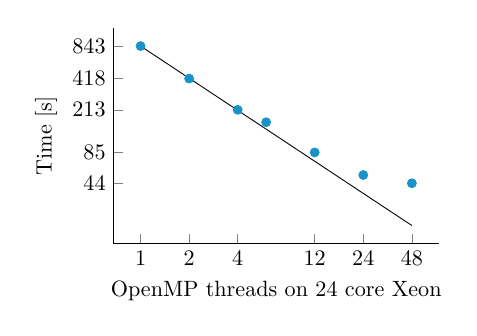
\begin{tikzpicture}[scale=.8]
	\begin{loglogaxis}[
	axis x line*=bottom,
	axis y line*=left,
	xlabel={OpenMP threads on 24 core Xeon},
	ylabel={Time [s]},
	width=6.75cm,
	height=5cm,
	log ticks with fixed point,
	xtick={1,2,4,12,24,48},
	ytick={44,85,213,418,843}
	]
	\addplot[domain=1:48] {843/x};
	\addplot [color=ACATlblue, only marks] coordinates {%
		(1,843)
		(2,418)
		(4, 213)
		(6,163)
		(12, 84.98)
		(24, 52.22)
		(48,43.7)
	};
	
	\end{loglogaxis}
	\end{tikzpicture}
	
	\begin{block}{$\pi\pi\pi^0$, 16 time-dependent amplitudes}
		\begin{itemize}
			%			\item 40 free par.\ and 100,000+ events
			\item Original RooFit code: \unit[19,489]{s} single core
		\end{itemize}
		
		\vspace{-2.5ex}
		\begin{center}
			\begin{tabular}{r|r|l}
				2 Cores & Core 2 Duo &  \unit[1,159]{s} \\
				GPU & GeForce GTX 1050 Ti &  \unit[86.4]{s} \\
				GPU & Tesla K40 & \unit[64.0]{s} \\
				MPI & Tesla K40 $\times 2$ & \unit[39.3]{s} \\
				GPU & Tesla P100 &  \unit[20.3]{s}
				% 3 cards: 34.8 s
				% 2 K-40s: 39.3 s
			\end{tabular}
		\end{center}
	\end{block}
	
	\column{.5\textwidth}
	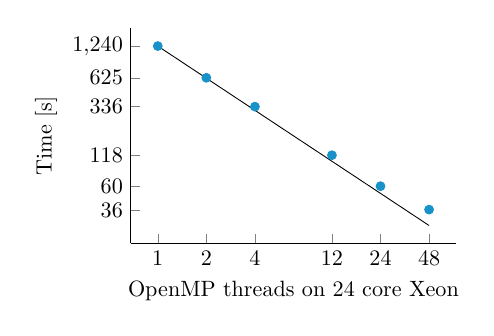
\begin{tikzpicture}[scale=.8]
	\begin{loglogaxis}[
	axis x line*=bottom,
	axis y line*=left,
	xlabel={OpenMP threads on 24 core Xeon},
	ylabel={Time [s]},
	width=6.75cm,
	height=5cm,
	log ticks with fixed point,
	xtick={1,2,4,12,24,48},
	ytick={36, 60, 118, 336, 625, 1240}
	]
	\addplot[domain=1:48] {1239.565/x};
	\addplot [color=ACATlblue, only marks] coordinates {%
		(1,1239.5650)
		(2,625.0800)
		(4,335.6160)
		(12,117.7198)
		(24,60.3316)
		(48,36.4039)
	};
	
	\end{loglogaxis}
	\end{tikzpicture}
	
	\begin{block}{ZachFit: $M (D^{*+})-M (D^0)$}
		\begin{itemize}
			\item 142,576 events in unbinned fit
			%		\item 24 physical Xeon cores for plot(s)
		\end{itemize}
		\vspace{-2.5ex}
		\begin{center}
			\begin{tabular}{r|r|l}
				2 Cores & Core 2 Duo &  \unit[738]{s} \\
				GPU & GeForce GTX 1050 Ti & \unit[60.3]{s} \\
				GPU & Tesla K40 & \unit[96.6]{s} \\
				MPI & Tesla K40 $\times 2$ & \unit[54.3]{s} \\
				GPU & Tesla P100 & \unit[23.5]{s}
			\end{tabular}
		\end{center}
	\end{block}
\end{columns}
\begin{tikzpicture}[overlay, remember picture]
\node at (current page.north east)
[below left, xshift=-.2cm, yshift=-1.2cm, align=right,font=\scriptsize]
{%
	\href{http://inspirehep.net/record/1229331}{[Phys.Rev.Lett. 111 (2013) no.11, 111801]}\\
	\href{http://inspirehep.net/record/1441203}{[Phys.Rev. D93 (2016) no.11, 112014]}\\
    \href{http://inspirehep.net/record/1228910}{[Phys.Rev. D88 (2013) no.5, 052003]}\\
    \href{http://inspirehep.net/record/1302129}{[CHEP 2013]}
};

 % PPPi_0
 % ZachFit
\end{tikzpicture}
\end{frame}

\subsection{How GooFit Works}
\begin{frame}{How GooFit Works}
    \begin{center}
        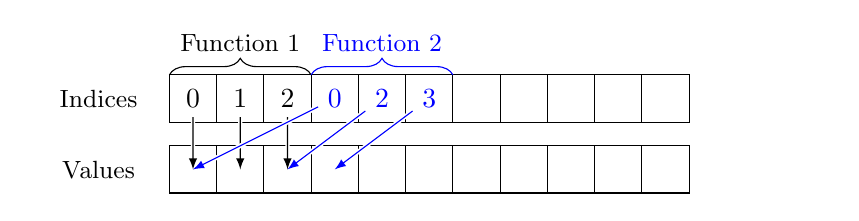
\begin{tikzpicture}[scale=.6,
            arr/.style={-latex, preaction={draw, -latex, white, ultra thick}}]
            \path[use as bounding box] (-3,-1.5) rectangle (14, 2);

            \foreach \x in {0,...,10} {
                \draw (\x,0) rectangle (\x+1,1);
                \draw (\x,-1.5) rectangle (\x+1,-.5);
            }
            \node at (-1.5,.5) {\small Indices};
            \node at (-1.5,-1) {\small Values};
            
            \node (a) at (0.5,.5) {0};
            \coordinate (A) at (0.5, -1);
            \draw [arr] (a) -- (A);

            \node (b) at (1.5,.5) {1};
            \coordinate (B) at (1.5, -1);
            \draw [arr] (b) -- (B);

            \node (c) at (2.5,.5) {2};
            \coordinate (C) at (2.5, -1);
            \draw [arr] (c) -- (C);

            \draw [decorate, decoration={brace,amplitude=6pt},xshift=0pt,yshift=0pt]
            (0,1) -- (3,1) node [black,midway,yshift=.4cm] {\small Function 1};

            \only<2>{
                \node [blue] (d) at (3.5,.5) {0};
                \draw [blue, arr] (d) -- (A);

                \node [blue] (e) at (4.5,.5) {2};
                \draw [blue, arr] (e) -- (C);

                \node [blue] (f) at (5.5,.5) {3};
                \coordinate (D) at (3.5, -1);
                \draw [blue, arr] (f) -- (D);

                \draw [blue, decorate, decoration={brace,amplitude=6pt},xshift=0pt,yshift=0pt]
                (3,1) -- (6,1) node [blue,midway,yshift=.4cm] {\small Function 2};
            }

        \end{tikzpicture}
    \end{center}
    \begin{columns}[c]
        \column{.65\textwidth}
        \begin{block}{How GooFit Works}
            \begin{itemize}
                \item CPU classes: Variable, Observable, DataSet, GooPdf
                \item Functions in CUDA with pointers held by GooPdf
                \item Function and variable arrays populated by GooFit
                \item Evaluation runs through CUDA functions through pointers (one kernel)
                \item Launching is handled by Thrust
            \end{itemize}
        \end{block}
        \column{.35\textwidth}
        \begin{center}
            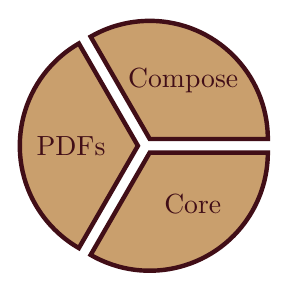
\begin{tikzpicture}
                \path [use as bounding box] (-1.5,-1.5) rectangle (1.5,1.5);
                \begin{scope}[xshift=0.5mm, yshift=0.866mm]
                    \path [ACATdark] (0,0) -- (0:1.5cm) arc (0:120:1.5cm) -- cycle;
                    \node [ACATdarktext] at (60:.85cm) {Compose};
                \end{scope}
                \begin{scope}[xshift=-1mm]
                    \path [ACATdark] (0,0) -- (120:1.5cm) arc (120:240:1.5cm) -- cycle;
                    \node [ACATdarktext] at (180:.85cm) {PDFs};
                \end{scope}
                \begin{scope}[xshift=0.5mm, yshift=-0.866mm]
                    \path [ACATdark] (0,0) -- (240:1.5cm) arc (240:360:1.5cm) -- cycle;
                    \node [ACATdarktext] at (310:.85cm) {Core};
                \end{scope}
            \end{tikzpicture}
        \end{center}
    \end{columns}
\end{frame}

\subsection{GooFit History}
\begin{frame}{GooFit History}
  
\begin{center}%
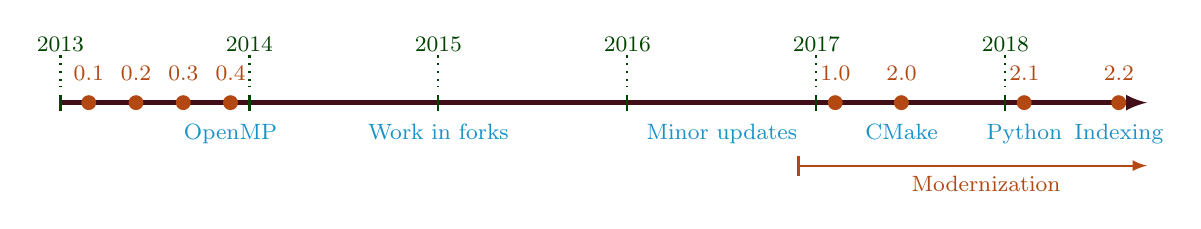
\begin{tikzpicture}[xscale=1.2,
	goonode/.style={fill=ACATdtan, circle, minimum size=1.25ex, inner sep=0},
	version/.style={above=1ex, ACATdtan},
	events/.style={below=1ex, ACATlblue},
	every node/.style={font=\footnotesize}
	]
	\draw [-latex, ultra thick, ACATdbrown] (0,0) -- (11.5,0);
	\draw [|-latex, thick, ACATdtan] (7.8,-.8) -- (11.5,-.8) node [midway, below, xshift=.5em] {Modernization};
	
	\foreach \x in {2013,...,2018} {
		\node at (2*\x-2*2013,0) [above=3.5ex, ACATdgreen] {\x};
		\draw [thick, ACATdgreen] (2*\x-2*2013,-.1) -- (2*\x-2*2013,.1);
		\draw [thick, dotted, ACATdgreen] (2*\x-2*2013,.6) -- (2*\x-2*2013,.2);
	}
	
	\node (v01) at (.3,0) [goonode] {};
	\node at (v01) [version] {0.1};
	
	\node (v02) at (.8,0) [goonode] {};
	\node at (v02) [version] {0.2};
	
	\node (v03) at (1.3,0) [goonode] {};
	\node at (v03) [version] {0.3};
	
	\node (v04) at (1.8,0) [goonode] {};
	\node at (v04) [events] {OpenMP};
	\node at (v04) [version] {0.4};
	
	\node at (4,0) [events] {Work in forks};
	
	\node (v10) at (8.2,0) [goonode] {};
	\node at (7,0) [events] {Minor updates};
	\node at (v10) [version] {1.0};
	
	\node (v20) at (8.9,0)  [goonode] {};
	\node at (v20) [events] {CMake};
	\node at (v20) [version] {2.0};

	\node (v21) at (10.2,0)  [goonode] {};
	\node at (v21) [events] {Python};
	\node at (v21) [version] {2.1};

	\node (v22) at (11.2,0)  [goonode] {};
	\node at (v22) [events] {Indexing};
	\node at (v22) [version] {2.2};
	\end{tikzpicture}%
\end{center}
\vspace{-.5cm}

  \begin{block}{Recent History}
    \begin{itemize}
      \item 2.0: New build system, C++11, and 4-body time dependent analyses support
      \item 2.1: Python bindings
      \item 2.2: New indexing (and lots of Python improvements)
    \end{itemize}
  \end{block}
\end{frame}

\section{GooFit and Python}
\subsection{Installation}
\begin{frame}{Installation (Python)}

    \begin{columns}[c]
        \column{.5\textwidth}
        \begin{block}{Pip install}
            \begin{itemize}
                \item Pip always builds from source
                \item Uses CUDA if found, otherwise OpenMP
                \item It is possible to pass in CMake arguments
            \end{itemize}
        \end{block}

        \begin{block}{Pip 9}
            \begin{itemize}
                \item \texttt{pip install skbuild cmake}
                \item \texttt{pip install -v goofit}
            \end{itemize}
        \end{block}

        \begin{block}{Pip 10}
            \begin{itemize}
                \item \texttt{pip install -v goofit}
                \item Note: not a formal endorsement of Pip 10
            \end{itemize}
        \end{block}

        \column{.5\textwidth}

        \begin{block}{CMake and normal directory}
            \begin{itemize}
                \item Use \texttt{GOOFIT\_PYTHON=ON} (\texttt{Auto})
                \item Build directory should be in path
            \end{itemize}
        \end{block}

        \begin{block}{Also available in repository}
            \begin{itemize}
                \item 12 of 13 C++ examples converted
                \item Interactive notebook examples
            \end{itemize}
        \end{block}
    \end{columns}
\end{frame}


\subsection{Comparison}
\begin{frame}[fragile]{Comparison}
    \begin{columns}[c]
        \column{.5\textwidth}
        \begin{lstlisting}[language=C++]
#include <goofit/...>
using namespace GooFit;

Observable x{"x", 0, 10};
Variable mu{"mu", 1};
Variable sigma{"sigma", 1, 0, 10};
GaussianPdf gauss{"gauss", &x, &mu, &sigma};
UnbinnedDataSet ds{x};

std::mt19937 gen;
std::normal_distribution<double> d{1, 2.5};
for(size_t i=0; i<100000; i++)
    ds.addEvent(d(gen));

gauss.fitTo(&ds);

std::cout << mu << std::endl;
\end{lstlisting}
        \column{.5\textwidth}
        \begin{lstlisting}[language=Python] 
from goofit import *
import numpy as np

x = Observable("x", 0, 10)
mu = Variable("mu", 1)
sigma = Variable("sigma", 1, 0, 10)
gauss = GaussianPdf("gauss", x, mu, sigma)
ds = UnbinnedDataSet(x)

data = np.random.normal(1, 2.5, (100000,1))
ds.from_matrix(data, filter=True)



gauss.fitTo(ds)

print(mu)
        \end{lstlisting}
    \end{columns}
\end{frame}

\subsection{Pythonisms}
\begin{frame}[fragile]{Pythonisms}
    \begin{columns}[c]
        \column{.5\textwidth}
        \begin{lstlisting}[language=Python]
mu.value = 2
print(mu)
        \end{lstlisting}
        \begin{block}{Variables}
            \begin{itemize}
                \item Variables provide property access
                \item Variables can be printed
            \end{itemize}
        \end{block}
        \begin{block}{Memory}
            \begin{itemize}
                \item GooFit object memory handled transparently
            \end{itemize}
        \end{block}
        \column{.5\textwidth}
        \begin{lstlisting}[language=Python]
ds.from_matrix(numpydata, filter=True)
        \end{lstlisting}
        \begin{block}{DataSet: from Python}
            \begin{itemize}
                \item DataSets can be read in/out to 2D buffers
                \item Option to filter invalid values
            \end{itemize}
        \end{block}
        \begin{lstlisting}[language=Python]
ds = BinnedDataSet(x, y, z)
ds.addEvent(xval, yval, zval)
        \end{lstlisting}
        \begin{block}{Arguments}
            \begin{itemize}
                \item Automatic conversion for lists
                \item Variable length arguments supported
            \end{itemize}
        \end{block}
    \end{columns}
\end{frame}

\subsection{Simulation}
\begin{frame}[fragile]{Simulation and Evaluation}
    \begin{columns}[c]
        \column{.5\textwidth}
        \begin{lstlisting}[language=Python]
grid, pts = gauss.evaluatePdf(x)
gauss.setData(grid)
        \end{lstlisting}
        \begin{block}{PDF evaluation}
            \begin{itemize}
                \item Evaluate on a grid
                \item Can be rerun interactively
            \end{itemize}
        \end{block}

        \begin{lstlisting}[language=Python]
gauss.fillMCDataSimple(1000000)
        \end{lstlisting}
        \begin{block}{1D MC generation}
            \begin{itemize}
                \item Simple way to produce MC
                \item Initial MC on CPU, evaluation on GPU
            \end{itemize}
        \end{block}
        \column{.5\textwidth}
        \begin{lstlisting}[language=Python]
dplt = DalitzPlotter(prod, dp)
arr = dplt.make2D()        
        \end{lstlisting}
        \begin{block}{Amp3Body (TD)}
            \begin{itemize}
                \item Can produce simple 3-body Toy MC
                \item DalitzPlotter functionality planned for merge into Amp3Body
            \end{itemize}
        \end{block}

        \begin{lstlisting}[language=Python]
aa.setGenerationOffset(0);
aa.GenerateSig(1000000);
        \end{lstlisting}
        \begin{block}{Amp4Body (TD)}
            \begin{itemize}
                \item Full GPU Toy MC using \href{https://github.com/GooFit/MCBooster}{MCBooster}
            \end{itemize}
        \end{block}
    \end{columns}
\end{frame}

\subsection{Evaluation Example}
\begin{frame}{Evaluation Example}
    \begin{columns}
        \column{.5\textwidth}%
        \only<1>{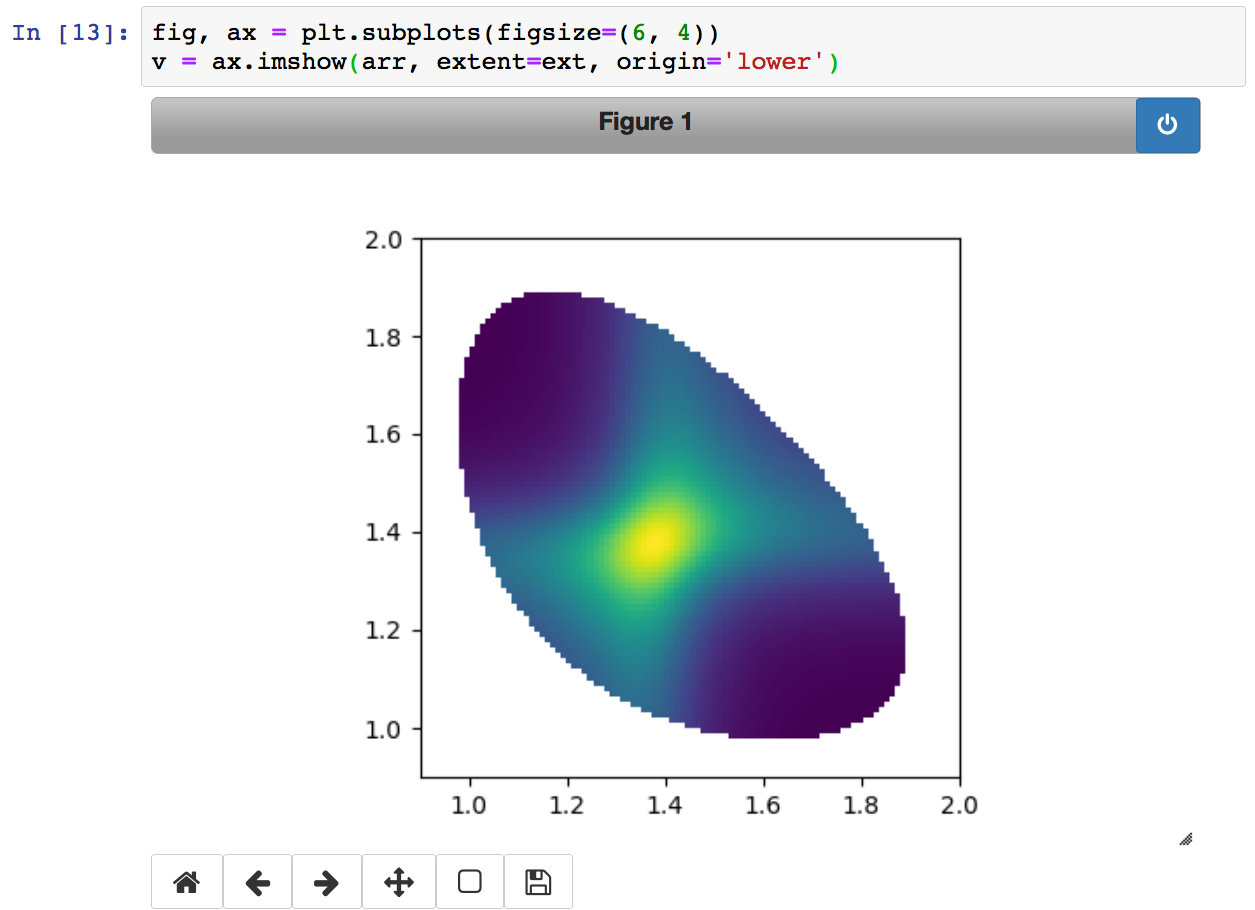
\includegraphics[width=\textwidth, trim={100 0 65 0}]{GooFitPlot1.png}}%
        \only<2>{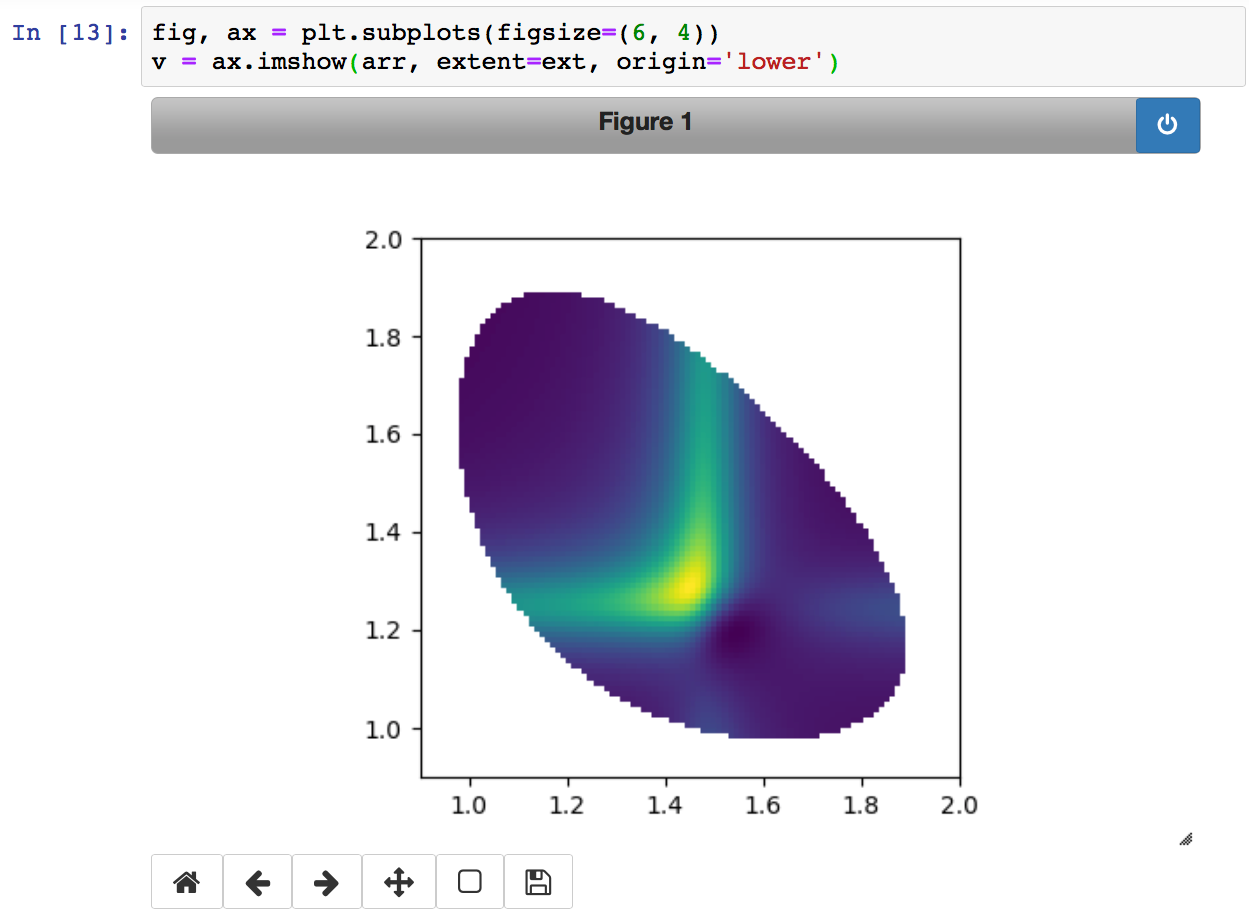
\includegraphics[width=\textwidth, trim={100 0 65 0}]{GooFitPlot2.png}}%
        \column{.5\textwidth}%
        \only<1>{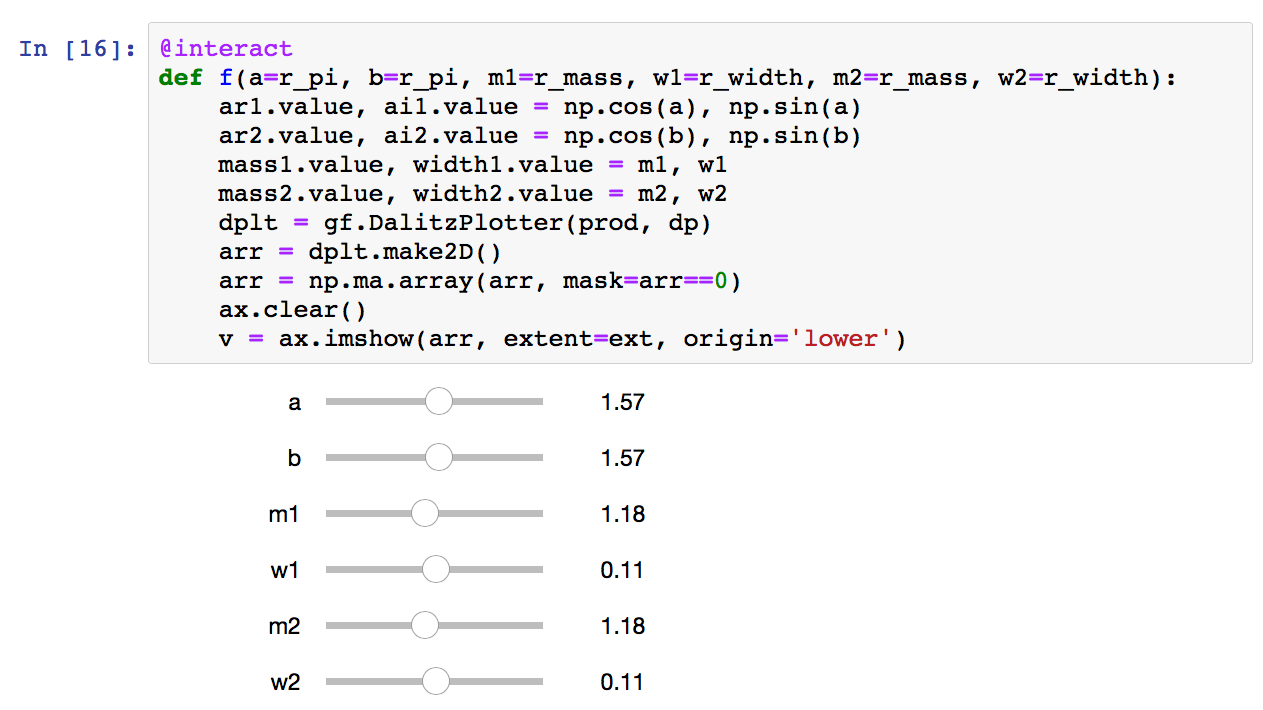
\includegraphics[width=\textwidth, trim={65 0 100 0}]{GooFitSliders1.png}}%
        \only<2>{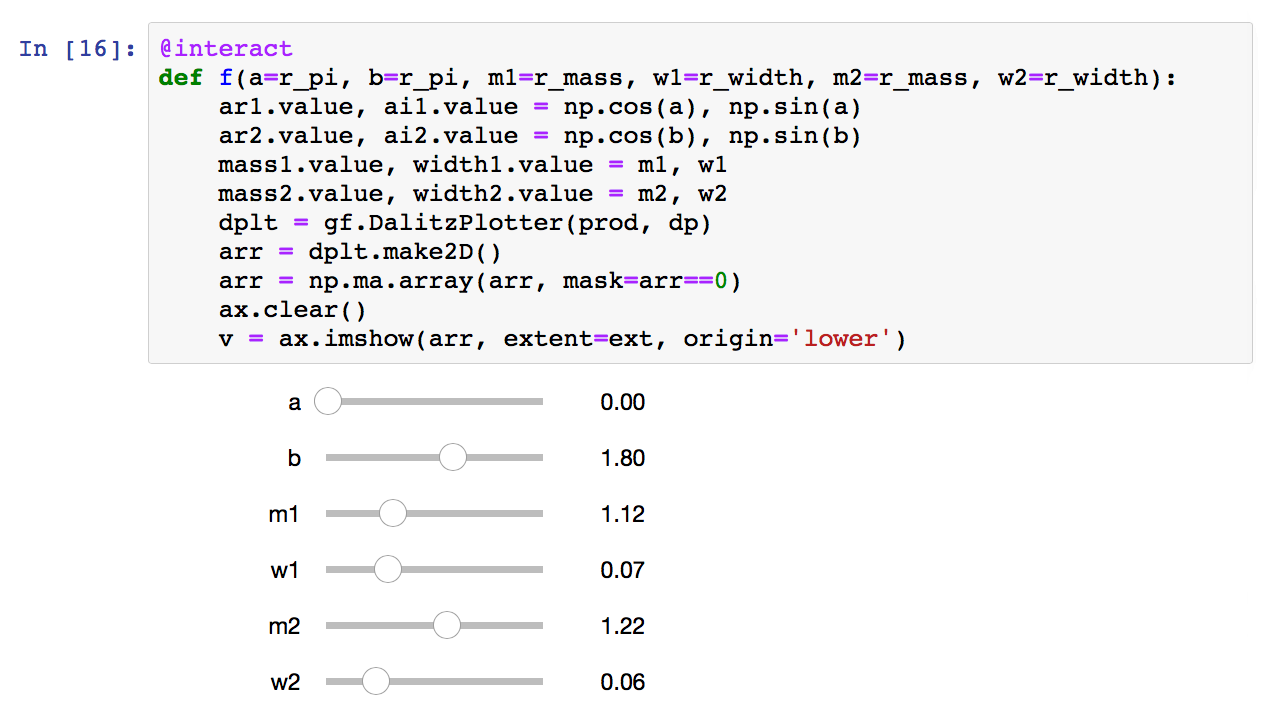
\includegraphics[width=\textwidth, trim={65 0 100 0}]{GooFitSliders2.png}}%
    \end{columns}
\end{frame}

\subsection{Documentation}
\begin{frame}[fragile]{Documentation}
    \begin{columns}[c]
        \column{.5\textwidth}
        \begin{block}{Documentation}
            \begin{itemize}
                \item Documentation exported to Jupyter
            \end{itemize}
        \end{block}
%\begin{lstlisting}[language=C++]
%.def_static("help", []() {
%    return HelpPrinter(MyPdf_docs);
%})
%        \end{lstlisting}
        \begin{block}{Implementation details}
            \begin{itemize}
                \item Generated by CMake from Doxygen style comments
                \begin{itemize}
                    \item Conversion to Jupyter style markdown for math
                \end{itemize}
                \item Attached to class in PyBind11
            \end{itemize}
        \end{block}
        \column{.5\textwidth}

        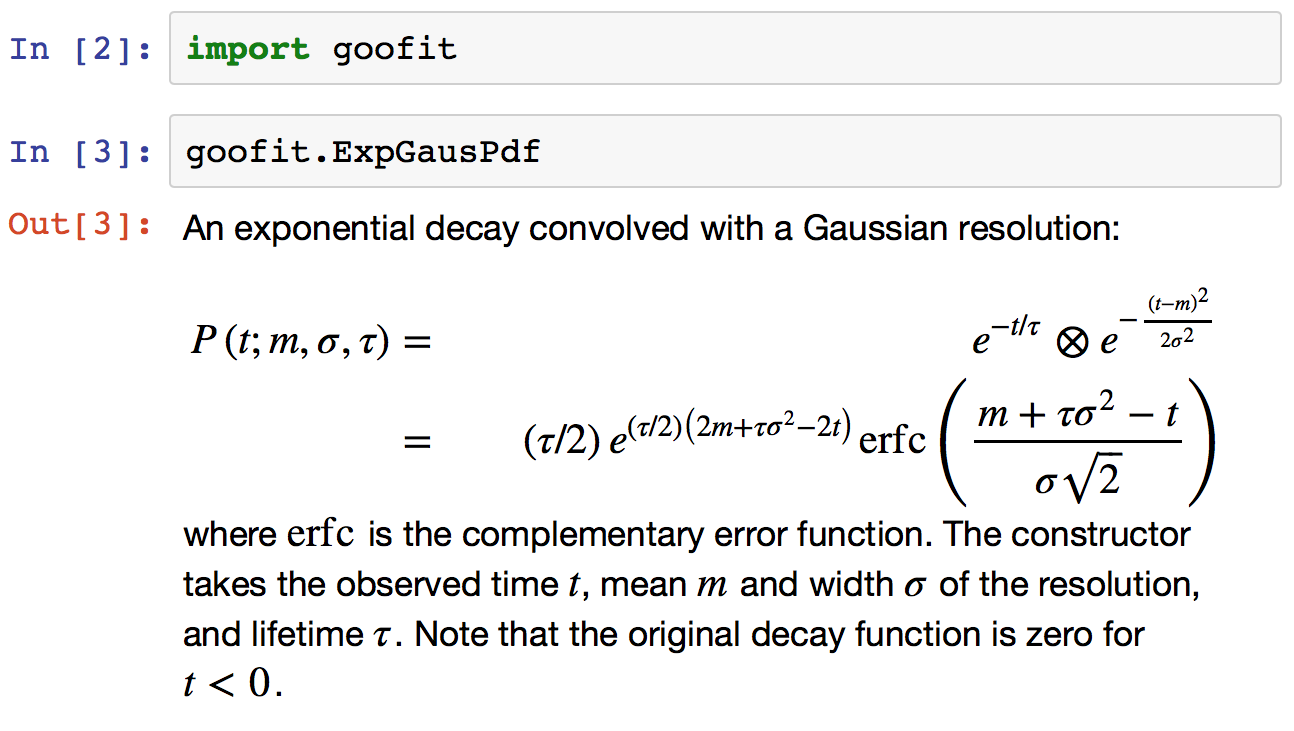
\includegraphics[width=\textwidth]{GooFitDocsExample}
    \end{columns}
\end{frame}

\section{Indexing}

\subsection{Device Indexing}
\begin{frame}[fragile]{Indexing in Device Functions}
\begin{lstlisting}[language=C++]
__device__ fptype f_device(fptype* evt, ParameterContainer& pc) {
    int id       = pc.getObservable(0);
    fptype x     = evt[id];
    fptype v     = pc.getParameter(0);
    pc.incrementIndex(1, 1, 0, 1, 1);
    return x * v;
}

__device__ device_function_ptr ptr_to_Gaussian = device_Gaussian;
\end{lstlisting}

\begin{block}{ParameterContainer}
    \begin{itemize}
        \item Simpler, easier device functions
        \item Faster on GPU, (currently) marginally slower on CPU
    \end{itemize}
\end{block}
\end{frame}

\subsection{Indexing in PDF}
\begin{frame}[fragile]{Indexing in PDF}
\begin{lstlisting}[language=C++]
 __host__ MyPdf::MyPdf(std::string name, Observable x, Variable v,)
     : GooPdf("MyPdf", name, x, v) {
     registerFunction("ptr_to_f", ptr_to_f);
     initialize();
 }
\end{lstlisting}

\begin{block}{Registration}
    \begin{itemize}
        \item Simply register the function (with debug name)
        \item Observables, Variables can be registered in the constructor
    \end{itemize}
\end{block}
\end{frame}

\section{AmpGen}
\subsection{Intro to AmpGen}
\begin{frame}{Introduction to AmpGen}
%    \begin{lstlisting}
%EventType D0 K- pi+ pi+ pi-
%D0[D]{K*(892)bar0{K-,pi+},rho(770)0{pi+,pi-}} 0 1 0.1 0 0 0.1
%K(1460)bar-_mass  0 1460 1 1000 2000
%K(1460)bar-_width 0  250 1 100  500
%a(1)(1260)+::Spline::Min 0.18412
%a(1)(1260)+::Spline::Max 1.86869
%    \end{lstlisting}
    \begin{columns}
        \column{.6\textwidth}
        \begin{block}{\href{https://gitlab.cern.ch/lhcb/Gauss/tree/LHCBGAUSS-1058.AmpGenDev/Gen/AmpGen}{AmpGen} by Tim Evans}
            \begin{itemize}
                \item Successor to MINT3: JIT compiler for amplitudes
                \item Includes easy to use and read grammar
                \item Inside LHCb framework, but can build standalone 
                \item Includes pure Python ctypes interface
            \end{itemize}
        \end{block}
        \column{.4\textwidth}
        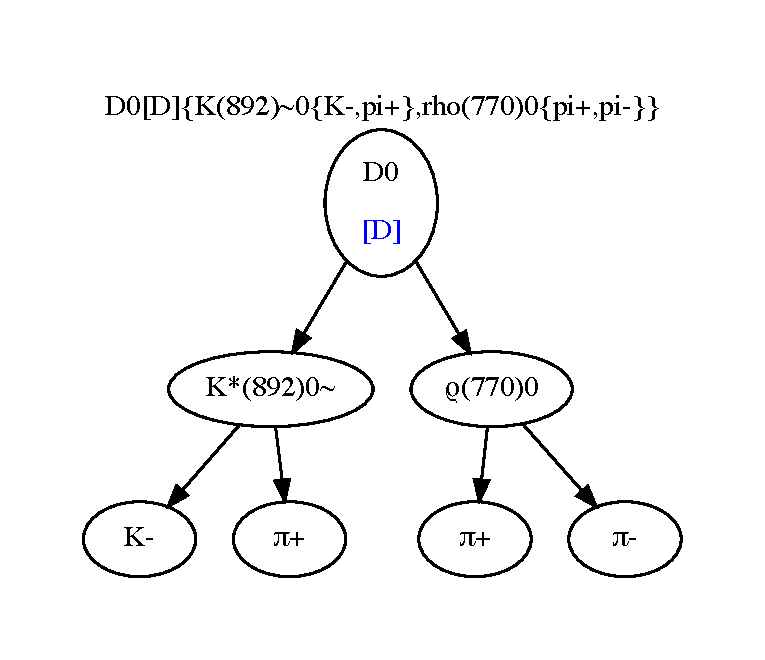
\includegraphics[width=\textwidth]{LineExample}
    \end{columns}
    
\end{frame}

\subsection{DecayLanguage}
\begin{frame}{DecayLanguage}
    \begin{columns}[c]
        \column{.6\textwidth}
        \begin{block}{\href{https://decaylanguage.readthedocs.io/en/latest/}{DecayLanguage}: BETA}
            \begin{itemize}
                \item Python package implementing AmpGen's syntax
                \item Reads in and understands decay chains
                \item Still in beta: future potential
                \item Can output GooFit code!
                \item On \href{https://pypi.org/project/decaylanguage/}{PyPI} and \href{https://decaylanguage.readthedocs.io/en/latest/}{ReadTheDocs}
            \end{itemize}
        \end{block}
        \column{.4\textwidth}
        $D^0\rightarrow K^{\mp} \pi^{\pm} \pi^{\pm} \pi^{\mp}$ model \href{https://inspirehep.net/record/1644791}{[Eur.Phys.J. C78 (2018)]}
        
        \begin{itemize}
            \item AmpGen model: 222 lines
            \item GooFit model: 1314 lines
        \end{itemize}
    \end{columns}
\end{frame}

\section{Final Words}
\subsection{Summary}
\begin{frame}{Summary}
    \begin{columns}[t]
        \column{.333333\textwidth}
        \begin{block}{GooFit Python}
            \begin{itemize}
                \item Easy to compose model
                \item Easy to manipulate model
                \item Pythonic interface
            \end{itemize}
        \end{block}
        \column{.333333\textwidth}
        \begin{block}{GooFit Indexing}
            \begin{itemize}
                \item Simpler to add PDFs
                \item Faster on GPU
                \item More flexibility for developers
            \end{itemize}
        \end{block}
        \column{.333333\textwidth}
        \begin{block}{AmpGen/DecayLanguage}
            \begin{itemize}
                \item Syntax for amplitudes
                \item Beta Python package
                \item Future potential
            \end{itemize}
        \end{block}
    \end{columns}
\end{frame}


\backupbegin
\section{Backup}

\subsection{Backup slides}


\backupend

\end{document}
